\documentclass[a4paper,14pt]{extarticle} \usepackage[utf8]{inputenc}
\usepackage[T1]{fontenc}
\usepackage[margin=2.5cm]{geometry}

% Fonte Caladea se existir, senão lmodern
\IfFileExists{caladea.sty}{
  \usepackage{caladea}
}{
  \usepackage{lmodern} }
\usepackage{ragged2e}
\usepackage{graphicx}
\usepackage[portuguese]{babel}
\usepackage{wrapfig}
\usepackage{hyperref}
\usepackage{fancyhdr}
\usepackage{xcolor}
\usepackage{rotating}
\usepackage{titlesec}
\usepackage{epigraph}
\usepackage{dirtytalk}
\usepackage{indentfirst} % Indenta o primeiro parágrafo após seções

% Ajuste do recuo de parágrafo
\setlength{\parindent}{1.5em}

% Centralizar títulos
\titleformat{\section}
  {\normalfont\centering\bfseries\Large}{\thesection}{1em}{}

\titleformat{\subsection}
  {\normalfont\centering\bfseries\large}{\thesubsection}{1em}{}

\titleformat{\subsubsection}
  {\normalfont\centering\bfseries}{\thesubsubsection}{1em}{}

% -------------- Símbolos de Versículo e Resposta --------------
% Definição do símbolo (a “barrinha” inclinada)
\makeatletter
\newcommand{\vers@resp@sym}{%
  \raisebox{0.2ex}{\rotatebox[origin=c]{-20}{$\m@th\rceil$}}%
}
% macro interna que sobrepõe a barrinha e a letra V ou R
\newcommand{\vers@resp}[2]{%
  {\ooalign{%
     \hidewidth\kern#1\vers@resp@sym\hidewidth\cr
     #2\cr
  }}%
}
% comandos públicos \versicle e \response
\DeclareRobustCommand{\versicle}{\vers@resp{-0.1em}{V}}
\DeclareRobustCommand{\response}{\vers@resp{0pt}{R}}
\makeatother
% ^------------- Símbolos de Versículo e Resposta -------------^

% Rodapé com imagem e página
\pagestyle{fancy}
% ---- Cabeçalho ------------
\fancyhf[C]{}
% ----- Rodapé --------------
\fancyfoot[LO,LE]{%
  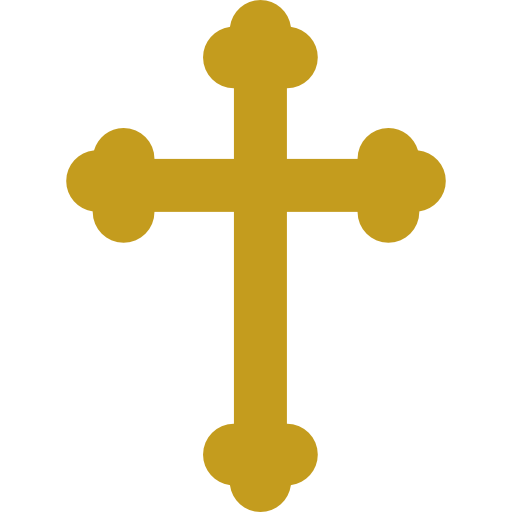
\includegraphics[scale=0.2]{assets/cross.png}\quad
  \textit{Novena a \textbf{São Nuno de Santa Maria}}
}
\fancyfoot[RO,RE]{\thepage}

\begin{document}


\begin{center}
  {\huge Novena a São Nuno de Santa Maria}
\end{center}

\par\noindent\rule{\textwidth}{0.4pt}

\tableofcontents
\thispagestyle{empty}

% --- Vida / Origem da Novena ---
\newpage

\section{História do Santo}
Nuno Álvares Pereiranasceu em Portugal a 24 de Junho de 1360, muito provavelmente em Cernache do Bonjardim, sendo filho ilegítimo de fr. Álvaro Gonçalves Pereira, cavaleiro dos Hospitalários de S. João de Jerusalém e Prior do Crato, e de D. Iria Gonçalves do Carvalhal. Cerca de um ano após o seu nascimento o menino foi legitimado por decreto real, podendo assim receber a educação cavalheiresca típica dos filhos das famílias nobres do seu tempo. Aos treze anos torna-se pajem da rainha D. Leonor, tendo sido bem recebido na Corte e acabando por ser pouco depois cavaleiro. Aos dezasseis anos casa-se, por vontade de seu pai, com uma jovem e rica viúva, D. Leonor de Alvim. Da sua união nascem três filhos, dois do sexo masculino, que morrem em tenra idade, e uma do sexo feminino, Beatriz, a qual mais tarde viria a desposar o filho do rei D. João I, D. Afonso, primeiro duque de Bragança.

Quando o rei D. Fernando I morreu a 22 de Outubro de 1383 sem ter deixado filhos varões, o seu irmão D. João, Mestre de Avis, viu-se envolvido na luta pela coroa lusitana, que lhe era disputada pelo rei de Castela por ter desposado a filha do falecido rei. Nuno tomou o partido de D. João, o qual o nomeou Condestável, isto é, Comandante supremo do exército. Nuno conduziu o exército português repetidas vezes à vitória, até se ter consagrado na batalha de Aljubarrota (14 de Agosto de 1385), a qual acaba por determinar à resolução do conflito.

Os dotes militares de Nuno eram no entanto acompanhados por uma espiritualidade sincera e profunda. O amor pela eucaristia e pela Virgem Maria são a trave-mestra da sua vida interior. Assíduo à oração mariana, jejuava em honra da Virgem Maria às quartas-feiras, às sextas, aos sábados e nas vigílias das suas festas. Assistia diariamente à missa, embora só pudesse receber a eucaristia por ocasião das maiores solenidades. O estandarte que elegeu como insígnia pessoal traz as imagens do Crucificado, de Maria e dos cavaleiros S. Tiago e S. Jorge. Fez ainda construir às suas próprias custas numerosas igrejas e mosteiros, entre os quais se contam o Carmo de Lisboa e a Igreja de S. Maria da Vitória, na Batalha.

Com a morte da esposa, em 1387, Nuno recusa contrair novas núpcias, tornando-se um modelo de pureza de vida. Quando finalmente se alcançou a paz, distribui grande parte dos seus bens entre os seus companheiros, antigos combatentes, e acabo por se desfazer totalmente daqueles em 1423, quando decide entrar no convento carmelita por ele fundado, tomando então o nome de frei Nuno de Santa Maria. Impelido pelo Amor, abandona as armas e o poder para revestir-se da armadura do Espírito recomendada pela Regra do Carmo: era a opção por uma mudança radical de vida em que sela o percurso da fé autêntica que sempre o tinha norteado. Embora tivesse preferido retirar-se para uma longínqua comunidade de Portugal, o filho do rei, D. Duarte, de tal o impediu. Mas ninguém pode proibir-lhe que se dedicasse a pedir esmola em favor do convento e sobretudo dos pobres, os quais continuou sempre a assistir e a servir. Em seu favor organiza a distribuição quotidiana de alimentos, nunca voltando as costas a um pedido. O Condestável do rei de Portugal, o Comandante supremo do exército e seu guia vitorioso, o fundador e benfeitor da comunidade carmelita, ao entrar no convento recusa todos os privilégios e assume como própria a condição mais humilde, a de frade Donato, dedicando-se totalmente ao serviço do Senhor, de Maria —a sua terna Padroeira que sempre venerou—, e dos pobres, nos quais reconhece o rosto de Jesus.

Significativo foi o dia da morte de frei Nuno de Santa Maria, o domingo de Páscoa, 1 de Abril de 1431, passando imediatamente a ser reputado de “santo” pelo povo, que desde então o começa a chamar “Santo Condestável”.

Mas, embora a fama de santidade de Nuno se mantenha constante, chegando mesmo a aumentar, ao longo dos tempos, o percurso do processo de canonização será bem mais acidentado. Promovido desde logo pelos soberanos portugueses e prosseguido pela Ordem do Carmo, depara com numerosos obstáculos, de natureza exterior. Foi somente em 1894 que o Pe. Anastasio Ronci, então postulador geral dos Carmelitas, consegue introduzir o processo para o reconhecimento do culto do Beato Nuno “desde tempos imemoriais”, acabando este por ser felizmente concluído, apesar das dificuldades próprias do tempo em que decorre, no dia 23 de Dezembro de 1918 com o decreto Clementissimus Deus do Papa Bento XV.

As suas relíquias foram trasladadas numerosas vezes do sepulcro original para a Igreja do Carmo, até que, em 1961, por ocasião do sexto centenário do nascimento do Beato Nuno, se organizou uma peregrinação do precioso relicário de prata que as continha; mas pouco tempo depois é roubado, nunca mais tendo sido encontradas as relíquias que contivera, tendo sido depostos, em vez delas, alguns ossos que tinham sido conservados noutro lugar. A descoberta em 1966 do lugar do túmulo primitivo contendo alguns fragmentos de ossos compatíveis com as relíquias conhecidas reacendeu o desejo de ver o Beato Nuno proclamado em breve Santo da Igreja.

O Postulador Geral da Ordem, P. Felipe M. Amenós y Bonet, conseguiu que fosse reaberta a causa, que entretanto era corroborada graças a um possível milagre ocorrido em 2000. Tendo sido levadas a cabo as respectivas investigações, o Santo Padre, Papa Bento XVI, dispõe a 3 de Julho de 2008 a promulgação do decreto sobre o milagre em ordem à canonização e durante o Consistório de 21 de Fevereiro de 2009 determina que o Beato Nuno seja inscrito no álbum dos Santos no dia 26 de Abril de 2009.

% --- Orações Diárias ---
\newpage

\section{Novena a São Nuno de Santa Maria}

\subsection{Oração Inicial} \label{oracao-inicial}

Pelo sinal da Santa Cruz, livrai-nos Deus, Nosso Senhor, dos nossos inimigos. Em nome do Pai, e do Filho, e do Espírito Santo. Amém.

Oração ao Divino Espírito Santo

Vinde, Espírito Santo, enchei os corações dos vossos fiéis e acendei neles o fogo do vosso Amor.

\versicle. Enviai o vosso Espírito e tudo será criado.

\response. E renovareis a face da terra.

\textbf{Oremos:} Ó Deus, que instruístes os corações dos vossos fiéis com a luz do Espírito Santo, fazei que apreciemos retamente todas as coisas segundo o mesmo Espírito e gozemos sempre da sua consolação. Por Cristo, Senhor Nosso.
Amém.

\textbf{Ato de Contrição}

Meu Deus, porque sois infinitamente bom e vos amo de todo o meu coração, pesa-me de vos ter ofendido e, com o auxílio da Vossa Divina graça, proponho firmemente emendar-me e nunca mais vos tornar a ofender. Peço e espero o perdão das minhas culpas pela vossa infinita misericórdia. Amém.

\subsection{Orações de Cada Dia} \label{cotidie-oratio}

\subsubsection{Meditação do 1º Dia: Rejeitar o mal e fazer o bem}

São Nuno de Santa Maria nasceu em 24 de junho de 1360. A data foi esta, dia da festa de São João Batista. Quanto ao local, os historiadores estão divididos… Cernache, Ourém, Santarém ou Flor da Rosa, nos arredores do Crato.

Filho bastardo de Álvaro Gonçalves Pereira, Prior da Ordem Militar dos Hospitalários – ou do Crato –, foi legitimado por ato do rei D. Pedro I. Vivia na corte portuguesa com seu pai, de quem recebeu sólida formação, seu irmão Diogo e outros cavaleiros hospitalários.

Quando chegou a notícia da marcha do exército castelhano sobre Lisboa, Nuno, que ainda não tinha completado 13 anos, recebeu uma inesperada missão do rei D. Fernando: fazer um reconhecimento militar das forças inimigas. Cumprida a missão, disse ao rei: “Muita gente mal acaudelada; pouca gente com bom capitão, bem acaudelada, os poderia desbaratar.” Ou seja, os castelhanos eram muitos, mas mal comandados; um pequeno grupo, com um capitão valente, os venceria com facilidade.

Nuno havia percebido que, nas batalhas da vida, tudo depende do “capitão”.

Dois séculos mais tarde, no seu estilo inconfundível, Santa Teresa de Jesus dirá: “Estando presente tão bom amigo e tão generoso capitão, Jesus Cristo, tudo podemos suportar. Ele é ajuda e dá forças; nunca falta, é verdadeiramente amigo.” A tática “de tão generoso capitão” não é galvanizar as massas ululantes… passa antes por se dirigir ao coração de cada homem e de cada mulher.

Dizia o Papa Bento XVI: “Ressoa então oportuna como nunca a exortação de Jesus, escrita pelo evangelista Marcos: ‘Convertei-vos e acreditai no Evangelho’ (cf. Mc 1,15). O desejo sincero de Deus leva-nos a rejeitar o mal e a fazer o bem. Esta conversão do coração é, antes de tudo, dom gratuito de Deus, que nos criou para Si e, em Jesus Cristo, nos redimiu: a nossa verdadeira felicidade consiste em permanecer n’Ele (cf. Jo 15,3).”

Diz-me, tu que hoje comigo inicias esta novena de preparação da festa de São Nuno de Santa Maria: neste mundo complicado, cheio de guerras e de ódios, será mais eficaz combater o mal com o mal, ou seguir o nosso amoroso Capitão que passou pelo mundo fazendo o bem? Pede hoje a São Nuno de Santa Maria que te alcance a graça de “permanecer em Jesus”, como ramo bem enxertado na cepa (cf. Jo 15,5).


\subsubsection{Meditação do 2º Dia: Obediente e fiel, desinstalado e pronto!}

Nuno viveu muito próximo do rei D. Fernando desde os 12 anos. Já armado cavaleiro, aos 16 anos sai da corte para casar… Por obediência, não rejeita a proposta de seu pai, apoiada pelo rei. A noiva estava escolhida: D. Leonor Alvim, uma viúva ainda jovem, fidalga de Pedraça, nas terras de Basto. Casou-se em 15 de agosto de 1376. O casamento ficou dissolvido por morte de D. Leonor, no ano de 1387. Dessa união nasceu uma menina, Beatriz, que viria a casar com o 1º Duque de Bragança, bastardo de D. João I.

A obediência às instâncias paternas leva D. Nuno a um casamento que não estaria nos seus projetos. Porém, assume o compromisso com fidelidade. Tu, que te dispuseste a fazer comigo esta novena, deixa que te interpele: como tens vivido estas virtudes da obediência e da fidelidade, sobretudo na tua relação com a Igreja?

Foram sete anos tranquilos que D. Nuno viveu em terras de Entre-Douro-e-Minho. Com a mulher que o amava e a filha Beatriz, o seu enlevo. Num local paradisíaco e com o conforto que a fidalga de Pedraça, sua mulher, lhe proporcionava. Como se aplica bem aos anos vividos por D. Nuno Álvares Pereira no remanso de Pedraça, este trecho da Carta aos Filipenses:

“Alegrai-vos sempre no Senhor. Repito: alegrai-vos! Não vos inquieteis com nada! Em todas as circunstâncias apresentai a Deus as vossas preocupações, mediante a oração, as súplicas e a ação de graças. E a paz de Deus, que excede toda a inteligência, haverá de guardar vossos corações e vossos pensamentos, em Cristo Jesus. Além disso, irmãos, tudo o que é verdadeiro, tudo o que é nobre, tudo o que é justo, tudo o que é puro, tudo o que é amável, tudo o que é de boa fama, tudo o que é virtuoso e louvável, eis o que deve ocupar vossos pensamentos.” (Fl 4, 4.6-8)

Porque nunca descurou a sua vida espiritual, o conforto e a abastança não o alienaram, nem dos seus deveres de estado, nem das exigências da sua fé, nem das suas obrigações cívicas. Pede a São Nuno de Santa Maria a graça de um compromisso sério para com Deus, para com a família, para com a pátria.


\subsubsection{Meditação do 3º Dia: Tudo sacrifica por um ideal que vem do Céu…}

O rei D. Fernando morre em 1383, deixando o país mergulhado numa crise com origem na sucessão dinástica. D. Leonor Teles, a rainha, apressou-se a tomar o poder com o intuito de o entregar à filha, também chamada Beatriz – como a de D. Leonor e D. Nuno –, casada com o rei de Castela.

Essa pretensão de D. Leonor Teles foi mal recebida pelo povo, que a odiava, primeiro pela influência abusiva nos assuntos da governação, depois por ser infiel ao rei desde que se perdera de amores por João de Andeiro, um nobre galego da maior confiança do rei D. Fernando, que o nomeara Conde de Ourém.

D. Nuno, perante o que acontecia na capital, deixa o conforto de Pedraça e vem para Lisboa juntar-se à gente sem pergaminhos, à arraia-miúda, ao “povo, povão”, aos homens bons, entre eles alguns fidalgos de linhagem, que querem Portugal – gente congregada em torno do Mestre de Avis, D. João, filho ilegítimo de D. Pedro I, portanto irmão do falecido rei D. Fernando.

A nobreza mais influente, e os seus irmãos – Pedro, o mais velho, que sucedera ao pai como Prior do Crato, e Diogo –, aceitaram como um fato consumado a coroação de D. Beatriz como rainha de Portugal.

D. Nuno acredita que lutar pela independência de Portugal corresponde à vontade de Deus. Ele, com seu braço forte, ajudará aqueles que ousarem este combate desigual. Descreve assim a sua luta:

“Vejo no meu entendimento um poço muito alto e muito profundo, cheio de grande escuridão; e bem me diz a vontade que não há homem que nele salte que dele possa escapar, salvo por grande milagre, querendo-o Deus livrar dele por sua mercê. E não posso com o meu coração senão que salte nele.”

Consciente da sua fragilidade para travar o combate, mas cheio de confiança no poder de Deus, D. Nuno Álvares Pereira saltou!

Tu, que comigo fazes esta novena… no seu 3º dia, faço-te uma provocação: alguma vez renunciaste a alguma vantagem por um ideal elevado, por uma convicção inalienável? Vê como D. Nuno deixou a mulher e a filha em terras de Basto, renunciou à amizade dos próprios irmãos, para lutar por um ideal, por Portugal! Pede a sua intercessão: que te alcance a graça de uma consciência bem formada e a perseverança na defesa de ideais elevados!


\subsubsection{Meditação do 4º Dia: Uma fé prática, vivida e testemunhada no dia a dia}

Em 1384, o rei de Castela entrou por Portugal adentro e pôs cerco a Lisboa. Porém, o povo resistiu heroicamente, não apenas nas ruas de Lisboa, mas também no Porto e em muitas outras terras do país, com particular vigor nas do Alentejo.

O Mestre de Avis havia nomeado Nun’Álvares “Fronteiro-Mor do Alentejo”, passando por cima do parecer de D. João das Regras, que o considerava demasiado novo, ainda com a desvantagem de ter os seus dois irmãos, Pedro e Diogo, do lado do inimigo. D. João das Regras, credenciado jurista, teve, nas Cortes de Coimbra de 1385, um papel decisivo na aclamação do Mestre de Avis como rei de Portugal.

Quanto à nomeação de D. Nuno, não teve razão… Em 6 de abril de 1384, depois de fulminantes operações no Alentejo, vence a Batalha de Atoleiros, usando a tática do quadrado. Porém, mais importante que a tática militar utilizada, terá sido aquela que foi ditada pela fé, expressa nestas recomendações aos soldados:

“Que se encomendassem a Deus e à Virgem Maria, sua Madre, que os quisesse ajudar contra os seus inimigos, pois era justa a querela que tinham contra eles, e que tivessem firme fé que assim havia de ser.”

Avistado o inimigo, D. Nuno apeou-se do cavalo, ajoelhou e fez uma sentida oração ao crucifixo e à imagem da Santíssima Virgem estampados na sua bandeira. E com ele ajoelharam, comovidos, todos os soldados.

A ti, que aceitaste fazer comigo esta novena que vai no 4º dia… Que homem este, o nosso Santo Condestável! Deus e a Virgem Maria são a sua força; não esconde a sua fé; não tem respeitos humanos. Pede-lhe que te ajude a aplicar a sua tática nos combates interiores e exteriores que tens pela frente. Tantos e tão exigentes! Segue-lhe o exemplo: faz aquilo que podes fazer; suplica ajuda de Deus e a proteção da Mãe; acredita que Deus pode, e a Virgem ajuda!


\subsubsection{Meditação do 5º Dia: Quedo, em grande sossego… falava com Deus}

D. Nuno Álvares Pereira pacificou o Alentejo. Por sua vez, a peste dizimou muitos dos castelhanos que cercavam Lisboa; os que restaram, de mansinho, regressaram a Castela. Portugal aproveitou a trégua para resolver a questão dinástica. As Cortes de Coimbra, que tiveram início em março e terminaram no início de abril de 1385, confirmaram o querer do povo: que fizessem rei o Mestre de Avis.

A 6 de abril, 1º aniversário da vitória na Batalha de Atoleiros, D. João I é aclamado rei; nesse mesmo dia, nomeia D. Nuno Álvares Pereira Condestável do Reino, isto é, comandante supremo do exército português.

Resolvida a questão dinástica, permanecia em aberto o intrincado problema das relações com Castela… Os castelhanos, desta vez entrando pela Beira, avançavam de novo para Lisboa. D. Nuno Álvares Pereira não se intimidou: embora as suas forças estivessem em grande desvantagem numérica – 7.000 homens para 32.000 castelhanos bem armados –, bloqueou os castelhanos em Aljubarrota e, com uma capacidade de comando impressionante, em meia hora desbaratou o inimigo, infligindo-lhe humilhante derrota.

Foi o desfecho da Batalha de Aljubarrota, a 14 de agosto de 1385, véspera da Festa de Nossa Senhora da Assunção, dia de jejum que, tanto ele como os seus soldados, respeitaram. Ainda no rescaldo de Aljubarrota, o exército português encontrou-se com o de Castela perto de Mérida, na Batalha de Valverde, também ganha por D. Nuno.

Foi difícil, a vitória. Em determinada altura da peleja, os castelhanos já cantavam vitória perante a desorientação dos nossos soldados, que tinham perdido o rastro de D. Nuno, a quem procuravam, vivo ou morto, por todos os cantos. Encontraram-no entre dois penhascos, de joelhos por terra, braços erguidos e olhos no Céu. Os soldados pediram-lhe que voltasse ao campo de batalha, pois o apuro era grande. Só quando terminou a oração se levantou, robustecido pela força do próprio Deus.

Tu que comigo perseveras nesta novena a São Nuno de Santa Maria… Já te aconteceu, certamente, teres de combater contra forças superiores às tuas, experimentando na luta os teus limites. Nessas circunstâncias, passou-te pela cabeça parar um pouco, ajoelhar e olhar o Céu? E jejuar nas vésperas de uma prova importante, alguma vez o fizeste? Ou antes, nas dificuldades, continuas esbracejando, cheio de orgulho, querendo vencer apoiado nas tuas próprias forças? São Nuno venceu com jejum e oração… Pede-lhe que te alcance aquilo que precisas para vencer esse teu orgulho e cultivar a humildade.


\subsubsection{Meditação do 6º Dia: A devoção a Maria Santíssima leva a uma vida centrada em Deus}

Os dotes militares de Nuno eram, como temos visto nestas meditações, acompanhados por uma espiritualidade sincera e profunda. O amor à Eucaristia e à Virgem Maria são a trave-mestra da sua vida interior. Assíduo à oração mariana, jejuava em honra da Virgem Maria às quartas-feiras, às sextas, aos sábados e nas vigílias das suas festas. Assistia diariamente à Missa, embora só pudesse receber a Eucaristia por ocasião das maiores solenidades.

O estandarte que elegeu como insígnia pessoal traz as imagens do Crucificado, de Maria e dos cavaleiros São Tiago e São Jorge. É com a ajuda de Deus e a mediação de Maria Santíssima que D. Nun’Álvares Pereira prossegue o objetivo da paz com Castela. Conseguiu-o, finalmente, a 30 de outubro de 1411.

O prestígio do Condestável era imenso, tanto na corte como junto ao povo. As suas vitórias militares permitiram-lhe acumular riquezas e títulos, como o de Conde de Ourém, por nomeação do Mestre de Avis logo após a vitória na Batalha de Atoleiros. Embora D. Nuno fosse um homem sóbrio e modesto, ser Conde de Ourém dava-lhe um gozo especial…

Quando veio das Terras de Bouro para Lisboa, num curto retiro em Santarém, entregou aos cuidados de um alfageme a sua espada, para que a polisse e afiasse. O homem, na hora do pagamento, profetizou: “Não aceitarei qualquer pagamento senão quando o vir elevado a Conde de Ourém.” O Conde de Ourém era, na altura, o tal João de Andeiro, amante de D. Leonor Teles, que acabou sendo assassinado num golpe palaciano, pelo Mestre de Avis e seus apoiadores. O título deste traidor passou para D. Nuno, cumprindo-se a “profecia” do alfageme de Santarém, o que terá o feito pensar na célebre expressão popular: “A voz do povo é a voz de Deus.”

Conseguida a paz com Castela, o Condestável participa ainda, em 1415, na expedição a Ceuta, para dar um sinal a D. João I, pouco entusiasmado com aventuras expansionistas. D. Nun’Álvares Pereira, já retirado destas lides, aponta o caminho, ligando o seu nome ao primeiro passo dado por Portugal naquilo que virá a ser a expansão ultramarina.

Chegamos ao 6º dia da novena, e continuo a ter-te como companheiro nesta jornada de preparação para a festa de São Nuno de Santa Maria. Esta meditação foi longa… ainda assim, deixa-me que te lance, não uma, mas três interpelações:

1. Acreditas que, não raras vezes, é através dos simples, como o alfageme de Santarém, que Deus nos fala, nos ensina, nos consola?
2. Já reparaste como São Nuno, apesar dos seus muitos e decisivos afazeres, tem um programa para a sua vida espiritual? E tu? Sempre a ratear o tempo para Deus ao tempo que Deus te concede, não é verdade?
3. Já pensaste que, na sua ida até Ceuta, São Nuno foi um precursor da Igreja em saída. E tu? Bem instalado, não é?


\subsubsection{Meditação do 7º Dia: Santo Condestável e São Nuno de Santa Maria são o mesmo santo…}

A 26 de abril de 2009, D. Nuno Álvares Pereira, a quem há muito os portugueses reconheciam como o Santo Condestável, foi inscrito no álbum dos santos. A partir de então, na liturgia e na linguagem da Igreja, o nosso santo passou a ser designado por São Nuno de Santa Maria. Também no que diz respeito à iconografia, o elmo, a armadura, a espada, têm sido preteridos a favor da apresentação do santo com hábito de carmelita, um ar seráfico e abraçando um crucifixo.

Há até quem defenda que, não fora D. Nuno ter deposto as armas e tornar-se donato no Convento do Carmo, não teria sido inscrito no cânon dos santos. Nada mais errado… É santo quem, em cada circunstância da vida, procura corresponder à vontade de Deus. Outra coisa São Nuno não procurou: nos verdes anos, quando se preparava para ser cavaleiro; na sua vida de casado e pai de família; quando se juntou e assumiu responsabilidades entre aqueles que, contra a subjugação a Castela, sonhavam Portugal; e quando pegou em armas contra os que queriam matar este sonho que ele, arriscando a própria vida, ajudou a tornar realidade.

Depois, como carmelita, continuou a querer ser santo e, por isso, como sempre, imitou a Virgem Santíssima no seu “faça-se”! São João Paulo II, após a celebração do Grande Jubileu do Ano 2000, escreveu a Carta Apostólica Novo Millennio Ineunte. No n. 31, define a santidade como a “medida alta” da vida cristã ordinária. É bom que o cristão, à semelhança de São Nuno, aprenda a ganhar altura, não para voar para fora do seu quotidiano, mas para o viver com um amor sempre maior.

Na meditação de ontem, referimos as traves-mestras da espiritualidade do Santo Condestável. Ainda que brevemente, façamos referência à influência que nele teve, armado cavaleiro aos 16 anos, esse fato. A Cavalaria começou por ser um código marcial; porém, sem deixar de o ser, com o decorrer dos anos, desenvolveu um código de ética para o comportamento correto da nobreza nas mais diversas ocasiões. A partir do final do século XI, as qualidades cavalheirescas essenciais incluíam coragem, habilidade militar, honra, lealdade, justiça, boas maneiras e generosidade para com os menos afortunados.

A Igreja promoveu entusiasticamente a Cavalaria, incluindo no seu código a exigência de que os cavaleiros, a par da proteção dos mais fracos, jurassem defender a Igreja. Foi esta a escola de D. Nuno Álvares Pereira.

Vamos no 7º dia desta novena, que nos tem ajudado a descobrir São Nuno como modelo de santidade. Os chamamentos que Deus te vai fazendo são diversos daqueles que lhe fez, porque as circunstâncias e a época em que viveu são diferentes. Mas a santidade, em qualquer época, em quaisquer circunstâncias, realiza-se procurando fazer a vontade de Deus.

Queres ser santo? Preocupas-te em fazer a Vontade de Deus? Para São Nuno, foram muito importantes os meios de formação, nomeadamente a Cavalaria… Aproveitas alguns dos meios de formação que te são propostos? Quais? Pede a intercessão de São Nuno para que cresça em ti o desejo de ser santo.


\subsubsection{Meditação do 8º Dia: A fé era a raiz; a virtude, a coragem, o amor à Pátria, os ramos da árvore da sua vida}

Com a morte da esposa, D. Leonor Alvim, em 1387, Nuno, apesar de muito instado a fazê-lo, mesmo por D. João I, recusou contrair novas núpcias. Entregou a filha Beatriz aos cuidados da avó materna e, em 1388, inicia, em Aljubarrota, a construção da Capela de São Jorge; em Valverde, mandou construir o Mosteiro de Nossa Senhora do Vencimento, oferecido aos carmelitas com quem, no Alentejo, teve estreitas relações; em 1389, lança-se num empreendimento de maior vulto: o Convento do Carmo, em Lisboa. O convento e, sobretudo, a sua igreja, queria-a a maior e a mais bela, testamento da sua piedade, em louvor da Santíssima Virgem.

Na verdade, quando, em 1411, alcançou a paz com Castela, começou a orientar a sua vida para o convento. Distribuiu grande parte dos seus bens entre os seus companheiros, antigos combatentes; em 1422, reparte pelos seus três netos os seus títulos e domínios e, em 1423, acabou por se desfazer totalmente do que ainda lhe restava e entrou no convento carmelita por ele fundado, o Convento do Carmo, tomando então o nome de Frei Nuno de Santa Maria.

Por amor, lutou por Portugal, que, sem a sua valentia, teria entrado, talvez para sempre, na órbita de Castela; por amor, abandona as armas e o poder para revestir-se da armadura do Espírito recomendada pela Regra do Carmo.

Diz o cronista geral dos carmelitas: “Admirável foi este santo varão pelas muitas e especiais virtudes que cultivou, não só depois do divórcio que fez com o mundo, mas também antes de receber o hábito religioso.” E um outro seu biógrafo: “Deus foi sempre o ponto de referência dos seus atos. E era-o com tão acabada coerência e harmonia, com tão profunda e sólida unidade, que debalde se procura nele um hiato, uma solução de continuidade, uma linha de ruptura, entre o heroísmo e a santidade. Por isso, em Nun’Álvares, o combatente e o monge, o cavaleiro e o professo, são apenas duas faces de uma só existência, superiormente inspirada por um único ideal de serviço, o qual descia do coração de Deus para o coração dos homens.”

Estamos já, por graça de Deus, no 8º dia da nossa novena a São Nuno. Depois desta meditação, veio-me à memória aquela recomendação de Jesus que se cumpre no nosso santo: “Seja o vosso falar: sim, sim; não, não” (Mt 5,37). Não apenas o seu falar, mas, sobretudo, a sua vida foi sempre um “sim” a Deus e aos irmãos. Pede, por sua intercessão, a graça da unidade de vida. Ter uma vida para ir à Missa e outra para conviver com o mundo é coisa do maligno.


\subsubsection{Meditação do 9º Dia: \textit{“Ecce filius tuus}, Eis aí o teu filho”!}

O Condestável do Reino de Portugal, o comandante supremo do exército e seu guia vitorioso, o fundador e benfeitor do Convento do Carmo, ao professar como irmão leigo (frade donato), em 1423, recusou todos os privilégios, dedicando-se totalmente ao serviço do Senhor, de Maria e dos pobres, nos quais reconheceu sempre o rosto de Jesus.

Deixemos de novo falar o cronista geral dos carmelitas: “Depois de religioso, estreitou ainda mais o trato e familiaridade com o Senhor, porque então vivia no retiro conveniente para poder, sem estorvo, empregar todas as potências da alma no Divino Objeto que contemplava. Na presença da Virgem Maria, Senhora Nossa, com o título de Assunção, derramava copiosas lágrimas; e com elas, melhor do que com as vozes, Lhe apresentava as suas súplicas, para si e por aqueles que lhe pediam orações. Exemplaríssima foi sempre a humildade com que, antes e depois da vida religiosa, serviu a Deus. Foi admirável no exercício da caridade. Assistia os pobres e os enfermos, não só com o que era necessário, mas também com os mimos que conseguia.”

Debilitado nas forças físicas, percebeu que se aproximava a hora do seu último chamamento. Rogou que, para consolação do seu espírito, lhe lessem a Paixão de Cristo segundo São João; ao chegar àquela passagem em que Jesus, do alto da Cruz, entrega o discípulo amado à Sua Mãe, exalou, São Nuno, o último suspiro. Significativo foi o dia: o Domingo de Páscoa, 1º de abril de 1431.

Embora a fama de santidade de Nuno se tivesse mantido constante ao longo dos séculos, sendo o “Santo Condestável” como tal reconhecido pelo povo português desde tempos imemoriais, só foi beatificado em 23 de janeiro de 1918, pelo Papa Bento XV. O Santo Padre, Papa Bento XVI, durante o Consistório de 21 de fevereiro de 2009, determinou que o Beato Nuno fosse inscrito no cânon dos santos no dia 26 de abril de 2009. A sua memória litúrgica continuou a celebrar-se a 6 de novembro.




\subsection{Oração Final} \label{oracao-final}

Glorioso São Nuno de Santa Maria, orgulho do povo português, que escolheste como Mãe e celestial protetora, Aquela que é nossa Rainha e Padroeira; com o seu auxílio combateste o bom combate e sempre venceste as cobiças da terra; intercede por Portugal, para que permaneça fiel à santa Igreja; e desperta nos jovens o desejo da santidade! Confio-me à tua intercessão para que me alcances de Deus bom despacho na graça por que tanto anseio (\textbf{mencionar a graça…}). Amém.


\begin{center}
  Rezam-se 1 Pai Nosso, 3 Ave Marias, 1 Glória ao Pai.
\end{center}

\[
\textbf{São Nuno de Santa Maria, rogai por nós!}
\]

\vfill

\begin{center}
\subsection*{Fontes:}
Adaptado de: \underline{\href{https://bibliotecacatolica.com.br/blog/devocao/santo-inacio-de-antioquia/}{Minha Biblioteca Católica}} e \underline{\href{https://precantur.blogspot.com/2019/01/novena-ou-triduo-santo-inacio-de-antioquia.html}{Thesaurus Precantur}}.
\end{center}


\end{document}
